\section{Focussing the LMT}

\subsection{}
Like all telescopes, the LMT must be focused
several times a night. To do this we make a small map of a bright point-like source and then
adjust the z-position of the secondary mirror until the point spread function (the telescope’s
response function) is round and maximized. In this problem you will focus the telescope using
actual data taken on February 7, 2015.

The data is stored in the file maps.tar.gz on the class Moodle page. You can unpack that on
a linux computer with the commands: gunzip maps.tar.gz and tar -xcv maps.tar. This will
give you a set of 10 fits files (remember fits from homework 1) that you will read. The files
with “signal” in the name are the maps of the source. The files with "weight" in the name are
images with each pixel representing the weight $(1/\sigma^2)$ of each pixel in the corresponding signal
map.
Putting all this together, use the lmfit Levenberg-Marquardt fitting package to fit each image
to a 2-d gaussian. Find the best fit amplitude in each case and fit the best fit amplitudes to
the function
\begin{equation}
    f(z)=a_0+a_1z+a_2z^2
\end{equation}

where z is the z-position of the secondary as given in the table below. 
Use the results of this
fit to determine the best-fit position of the LMT's secondary mirror.

\begin{table}[h]
    \centering
    \begin{tabular}{|c|c|}
        \toprule
         Observation  & z-position (mm)  \\
         \midrule
         35114 & -3.0\\
         35115 & -2.0 \\
         35116 & -1.0 \\
         35117 & 0.0 \\
         35118 & 1.0\\
         \bottomrule
    \end{tabular}
    %\caption{Caption}
    %\label{tab:my_label}
\end{table}

\begin{figure*}
    \centering
    \begin{subfigure}[b]{.49\textwidth}
        \centering
        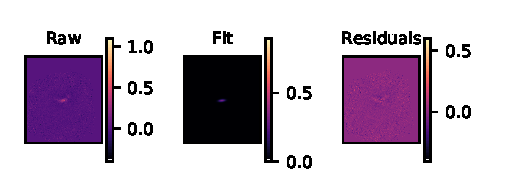
\includegraphics[height=100pt]{CodeAndFigures/DataFits4.pdf}
        \caption{Data:35114}
        \label{fig:lmtFit4}
    \end{subfigure}
    \begin{subfigure}[b]{.49\textwidth}
        \centering
        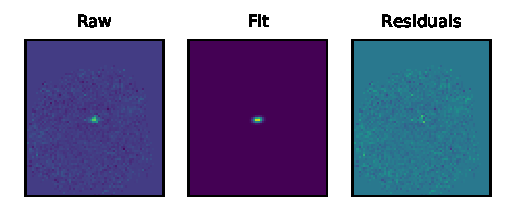
\includegraphics[height=100pt]{CodeAndFigures/DataFits5.pdf}
        \caption{Data:35115}
        \label{fig:lmtFit5}
    \end{subfigure}
    \begin{subfigure}[b]{.49\textwidth}
        \centering
        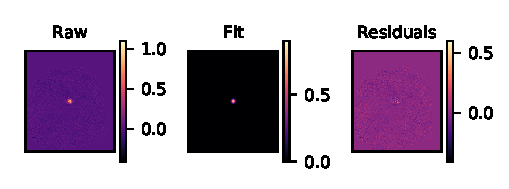
\includegraphics[height=100pt]{CodeAndFigures/DataFits6.pdf}
        \caption{Data:35116}
        \label{fig:lmtFit6}
    \end{subfigure}
    \begin{subfigure}[b]{.49\textwidth}
        \centering
        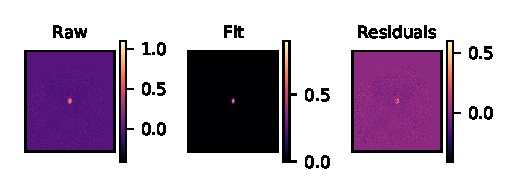
\includegraphics[height=100pt]{CodeAndFigures/DataFits7.pdf}
        \caption{Data:35117}
        \label{fig:lmtFit7}
    \end{subfigure}
    \begin{subfigure}[b]{.49\textwidth}
        \centering
        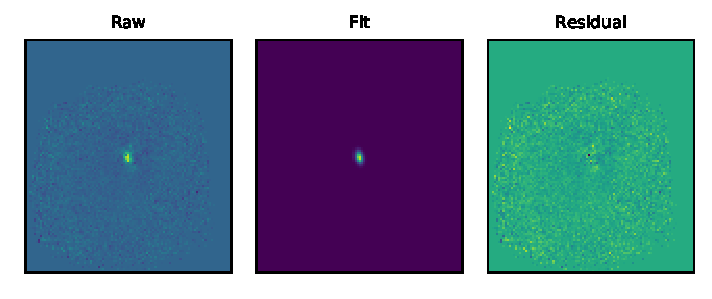
\includegraphics[height=100pt]{CodeAndFigures/DataFits8.pdf}
        \caption{Data:35118}
        \label{fig:lmtFit8}
    \end{subfigure}
    \caption{}
    \label{}
\end{figure*}


\subsection{}

Use either the procedure outlined in the class18 notes or the emcee
python package to simulate the posterior probability distributions for all of the fitted parameters
in one of the 2-d gaussian fits you did. Describe what you see.